\documentclass{beamer}

\mode<presentation>
{
  \usetheme{Madrid}      % or try Darmstadt, Madrid, Warsaw, ...
  \usecolortheme{crane} % or try albatross, beaver, crane, ...
  \usefonttheme{default}  % or try serif, structurebold, ...
  \setbeamertemplate{navigation symbols}{}
  \setbeamertemplate{caption}[numbered]
  
} 

\usepackage[english]{babel}
\usepackage[utf8x]{inputenc}
\usepackage{verbatim} 
\usepackage{caption}
\usepackage{multirow}
\usepackage{amsmath}
\usepackage{xcolor}
\usepackage[shortlabels]{enumitem}
\usepackage{subfigure}


\graphicspath{{img/}}

\newcommand{\vp}{\vspace{2mm}}
\newcommand{\xt}{\texttt}

\usepackage{color}
\providecommand{\pb}[1]{\textcolor{red}{#1}}
\providecommand{\cn}[1]{\textcolor{blue}{#1}}


\setitemize{label=\usebeamerfont*{itemize item}%
  \usebeamercolor[fg]{itemize item}
  \usebeamertemplate{itemize item}}


\title[Public Defense]{What You See is What You Get}
\subtitle{Methodological Component}
\author{Collin Nolte}
\date{March 8, 2023}

\begin{document}

\begin{frame}
  \titlepage
\end{frame}


\begin{frame}{Outline}\Large


\begin{itemize}
\item Mean structure assumptions
\item Alternative methods
  \begin{itemize}
  \item[--] Modified bootstrap
  \item[--] Permutation test
  \end{itemize}
\item FWER control
\item Power
\end{itemize}

\end{frame}

\begin{frame}{Mean Assumptions}\small
Observed data: \vspace{-2mm}
\begin{align*}
y_{it} = f(t|\theta_i) + \epsilon_{it}
\end{align*}

\underline{Homogeneous Means} \vspace{1mm}

For all subjects $i,j$ in group $g = 1, \dots, G$, \vspace{-4mm}

\begin{align*}
\theta_i = \theta_j
\end{align*}
\vspace{-4mm}


\underline{Heterogeneous Means} \vspace{1mm}

Subject $i$ in group $g = 1, \dots, G$ follows \vspace{-4mm}


\begin{align*}
\theta_i \sim N(\mu_g, V_g)
\end{align*}
\vspace{-4mm}
with no presumption that $\theta_i = \theta_j$

\end{frame}

\begin{frame}{Heterogeneous Bootstrap}
Differs from original \xt{bdots} bootstrap in that it samples subjects with replacement \vp

This gives distribution for the $b$th bootstrap estimate in group $g$
\begin{align*}
\theta_{bg}^{(het)} \sim N \left( \mu_{g}, \frac{1}{n_g} V_{g} + \frac{1}{n_g^2} \sum s_i^2 \right)
\end{align*}
This compares with homogeneous bootstrap which samples without replacement, 

\begin{align*}
\theta^{(hom)}_{bg} \sim N \left( \mu_{g}, \frac{1}{n_g^2} \sum s_i^2 \right).
\end{align*}

\end{frame}

\begin{frame}{Heterogeneous Bootstrap}
The change in algorithm (and resulting distribution) are only things that change \vp

Still construct test statistic

\begin{align*}
T_t = \frac{(\overline{p}_{1t} - \overline{p}_{2t})}{\sqrt{s_{1t}^2 + s_{2t}^2}}
\end{align*}
at each time point, with FWER being controlled with modified Bonferroni adjustment

\end{frame}


\begin{frame}{Permutation Test}
Begin by constructing test statistic on observed data,

\begin{align*}
T_t^{(p)} = \frac{|\overline{p}_{1t} - \overline{p}_{2t}|}{\sqrt{s_{1t}^2 + s_{2t}^2}}
\end{align*}
Then proceeded similarly to a standard permutation test by permuting labels for group membership at each permutation. At each permutation, retain the maximum test statistic, giving a null distribution of $P$ values denoted $\widetilde{T}$ \vp

Letting $\widetilde{T}_{\alpha}$ be the $1 - \alpha$ quantile of $\widetilde{T}$, significant regions will be those in which 
\begin{align*}
T_t^{(p)} \geq \widetilde{T}_{\alpha}
\end{align*}
\end{frame}


\begin{frame}{FWER Simulation}
\begin{itemize}
\item Logistic function from 0-1600
\item With and without AR(1) error
\item For heterogeneous means, sampled from empirical distribution from VWP with NH subjects
\item Paired data only for heterogeneous means, subjects differed only in error term
\item 25 subjects in each group (50 total), 100 simulations
\end{itemize}
\end{frame}

\begin{frame}{FWER Simulation}
\begin{figure}
\centering
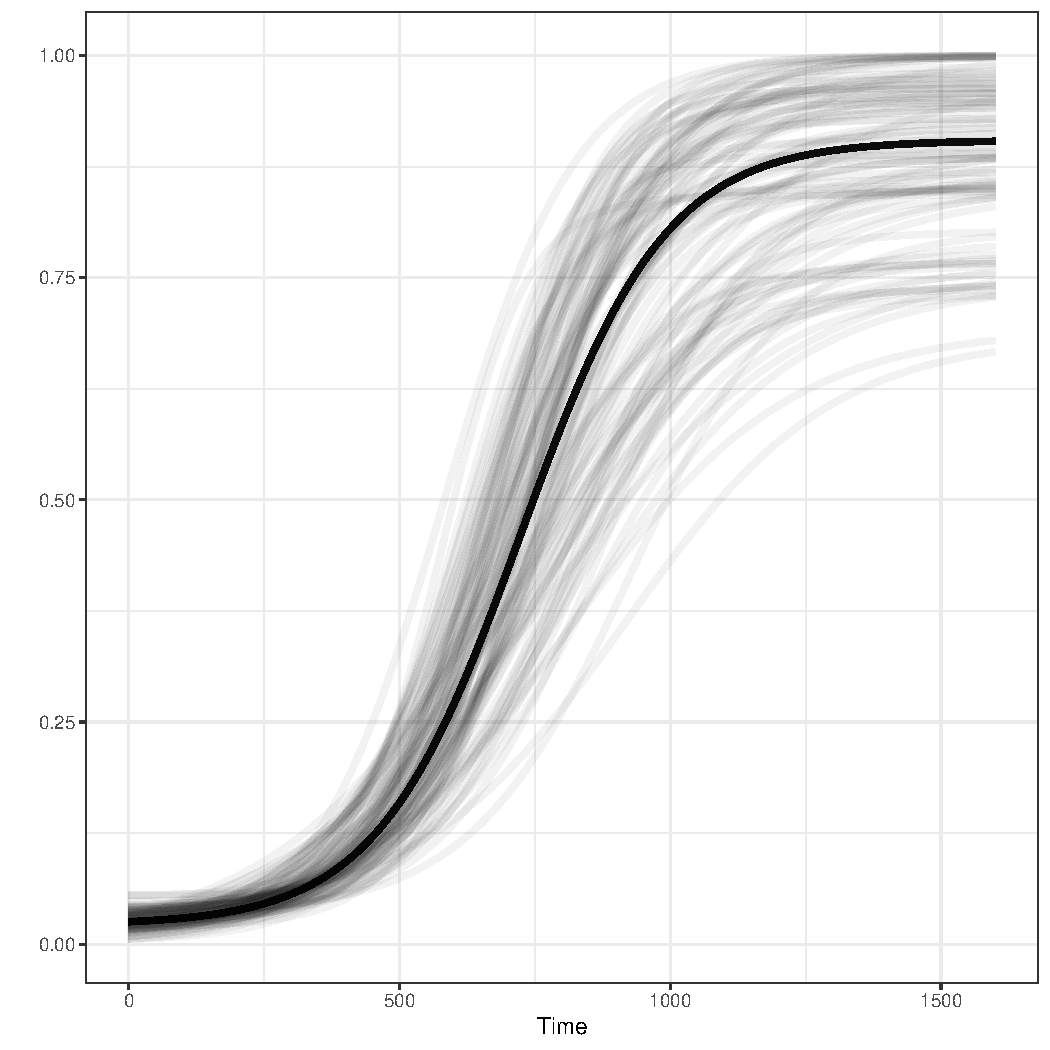
\includegraphics[scale = 0.4]{logistic_distribution.pdf}
\end{figure}
\end{frame}

\begin{frame}{FWER Results (Unpaired)}\small
\begin{table}[H]
\centering
\begin{tabular}{cccccc}
  \hline
  \multicolumn{1}{p{1.25cm}}{\centering $\theta_i = \theta_j$} & \multicolumn{1}{p{1.25cm}}{\centering AR \\ Error} & \multicolumn{1}{p{1cm}}{\centering AR(1)  \\ Specified} &  \multicolumn{1}{p{2cm}}{\centering Hom \\ Bootstrap} &\multicolumn{1}{p{2cm}}{\centering Het \\ Bootstrap} & \multicolumn{1}{p{2cm}}{\centering Permutation } \\ 
  \hline
No & Yes & Yes & 0.06 & 0.01 & 0.08 \\ 
  No & Yes & No & 0.87 & 0.08 & 0.00 \\ 
  No & No & Yes & 0.08 & 0.00 & 0.06 \\ 
  No & No & No & 0.15 & 0.02 & 0.01 \\ 
  Yes & Yes & Yes & 0.92 & 0.03 & 0.05 \\ 
  Yes & Yes & No & 0.96 & 0.02 & 0.08 \\ 
  Yes & No & Yes & 0.99 & 0.05 & 0.03 \\ 
  Yes & No & No & 1.00 & 0.05 & 0.06 \\  
   \hline
\end{tabular}
\caption{FWER for empirical parameters (unpaired)}
\label{tab:fwer_unpaired}
\end{table}
\end{frame}

\begin{frame}{FWER Results (Paired)}\small
\begin{table}[H]
\centering
\begin{tabular}{cccccc}
  \hline
  \multicolumn{1}{p{1.25cm}}{\centering $\theta_i = \theta_j$} & \multicolumn{1}{p{1.25cm}}{\centering AR \\ Error} & \multicolumn{1}{p{1cm}}{\centering AR(1)  \\ Specified} &  \multicolumn{1}{p{2cm}}{\centering Hom \\ Bootstrap} &\multicolumn{1}{p{2cm}}{\centering Het \\ Bootstrap} & \multicolumn{1}{p{2cm}}{\centering Permutation } \\ 
  \hline
  Yes & Yes & Yes & 0.49 & 0.02 & 0.01 \\ 
  Yes & Yes & No & 0.94 & 0.03 & 0.02 \\ 
  Yes & No & Yes & 0.72 & 0.02 & 0.00 \\ 
  Yes & No & No & 0.74 & 0.04 & 0.00 \\  
   \hline
\end{tabular}
\caption{FWER for empirical parameters (paired)}
\label{tab:fwer_unpaired}
\end{table}
\end{frame}

\begin{frame}{Power Simulation}
\begin{itemize}
\item Fit using piecewise function
\begin{align*}
y = \begin{cases}
b \quad &x < 0 \\
mx + b \quad &x \geq 0
\end{cases}
\end{align*}
\item cases with AR specification ugh
\item I have other sims that just aren't presented
\item 25 subjects in each group, 1000 simulations
\item Metrics include FWER, family wise type II error, and a distribution of where differences first detected (explain)
\end{itemize}
\end{frame}

\begin{frame}{Power Simulation}
\begin{figure}
\centering
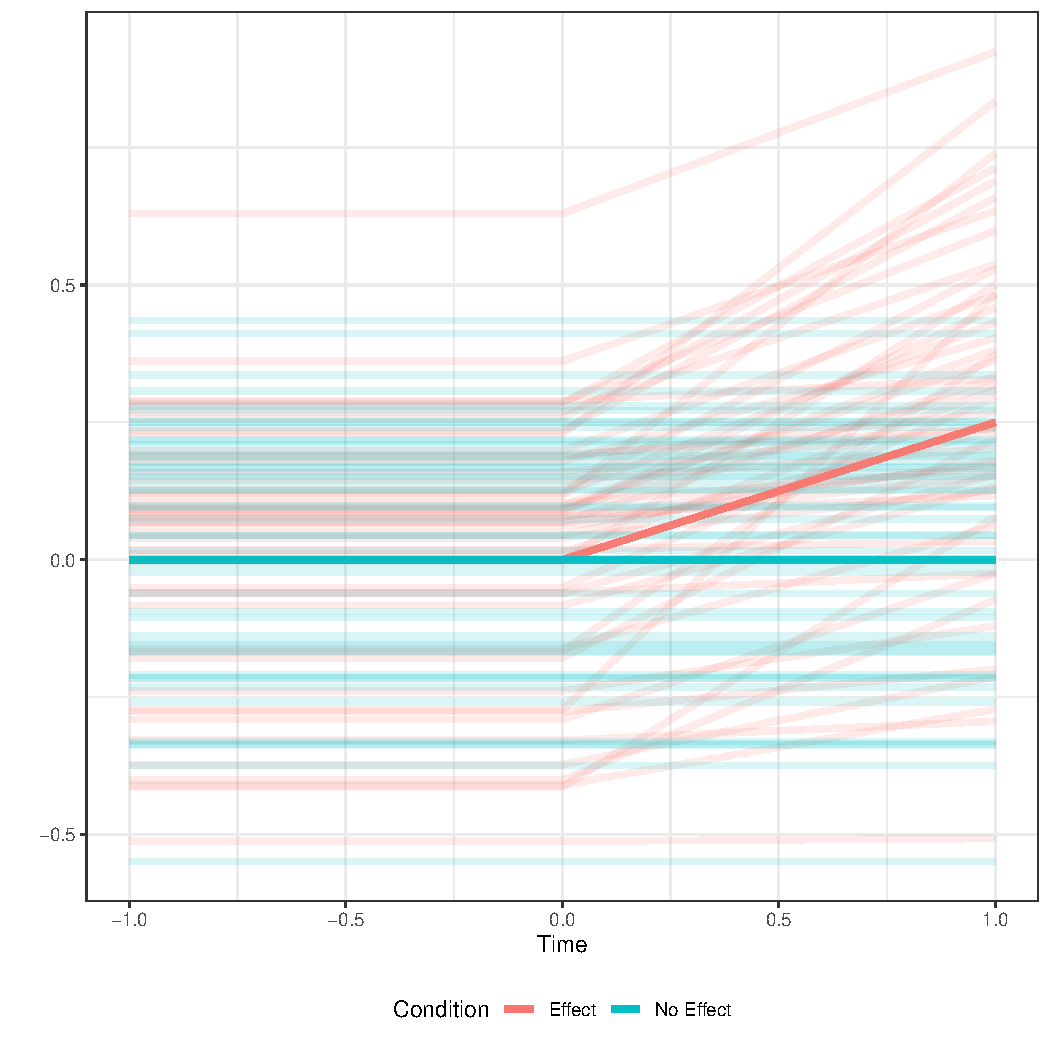
\includegraphics[scale = 0.4]{piecewise_distribution.pdf}
\end{figure}
\end{frame}

\begin{frame}{Power Results}\footnotesize
\begin{table}[H]
\centering
\begin{tabular}{lcccccccc}
  \hline
Method & Het. & AR(1) & $\alpha$ & $\beta$ & 1 - $\alpha$ - $\beta$ & 1st Qu. & Median & 3rd Qu. \\ 
  \hline
Hom. Boot & No & Yes & 0.00 & 0.00 & 1.00 & 0.025 & 0.030 & 0.035 \\ 
  Het. Boot & No & Yes & 0.00 & 0.00 & 1.00 & 0.035 & 0.040 & 0.045 \\ 
  Perm & No & Yes & 0.03 & 0.00 & 0.97 & 0.015 & 0.025 & 0.025 \\ 
  \hline
  Hom. Boot & Yes & No & 0.96 & 0.00 & 0.04 & 0.005 & 0.008 & 0.010 \\ 
  Het. Boot & Yes & No & 0.00 & 0.10 & 0.90 & 0.403 & 0.513 & 0.690 \\ 
  Perm & Yes & No & 0.03 & 0.05 & 0.92 & 0.378 & 0.515 & 0.681 \\ 
  \hline
  Hom. Boot & Yes & Yes & 0.97 & 0.00 & 0.03 & 0.008 & 0.010 & 0.010 \\ 
  Het. Boot & Yes & Yes & 0.01 & 0.10 & 0.89 & 0.420 & 0.525 & 0.690 \\ 
  Perm & Yes & Yes & 0.08 & 0.03 & 0.89 & 0.360 & 0.540 & 0.705 \\ 
   \hline
\end{tabular}
\caption{Power for methods} 
\label{tab:power_methods}
\end{table}
\end{frame}

\begin{frame}{Power (Homogeneous Means)}
\begin{figure}
\centering
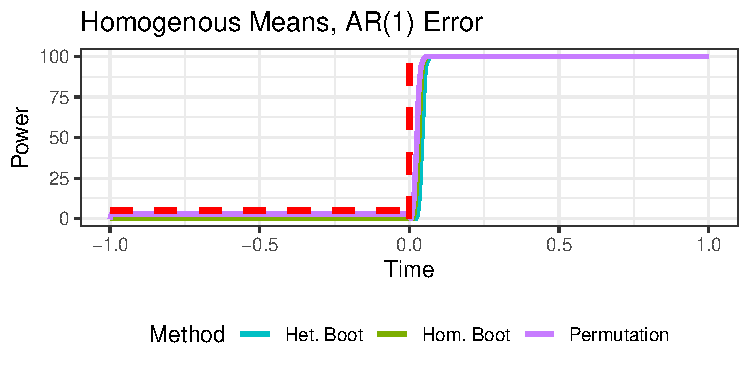
\includegraphics[width=0.9\textwidth]{type_two_error_time_a.pdf}
\end{figure}
\end{frame}

\begin{frame}{Power (Heterogeneous Means, AR(1))}
\begin{figure}
\centering
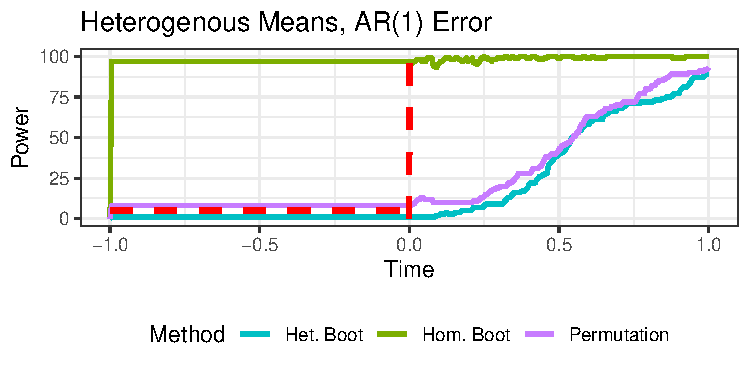
\includegraphics[width=0.9\textwidth]{type_two_error_time_b.pdf}
\end{figure}
\end{frame}


\begin{frame}{Power (Heterogeneous Means, No AR(1))}
\begin{figure}
\centering
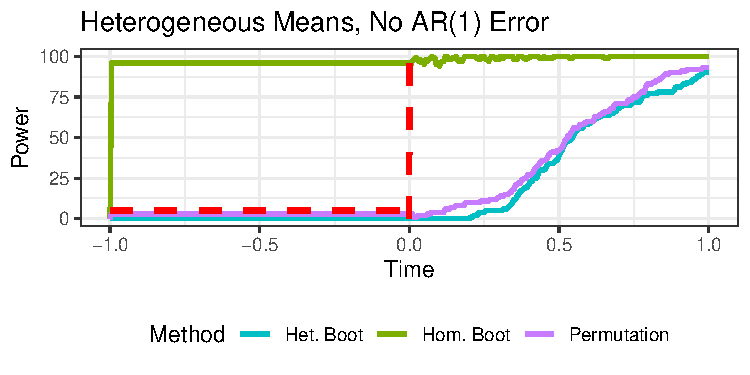
\includegraphics[width=0.9\textwidth]{type_two_error_time_c.pdf}
\end{figure}
\end{frame}



\begin{frame}{Conclusions}

\begin{itemize}
\item New methods adequately control FWER under myriad of situations
\item Also have comparable power under homogeneous means assumptions
\item In general, permutation performs closest to nominal alpha while having slightly improved power (compared to heterogeneous bootstrap)
\item Sampling without replacement will be removed from \xt{bdots} package as there is no situation in which is drastically outperforms any of the either two
\end{itemize}

\end{frame}

\end{document}